\state{\textit{H}-theorem and Pauli kinetic balance equation}{
	The Pauli balance equation (a version of the Boltzmann kinetic equation more suitable for a quantum setting) reads
	\eqn{Pauli}{
		\dwi = \sumj (\Pij \wj - \Pji \wi),
	}
	where $\wi$ is the probability of a system to be in the state $\ki$ and $\Pij$ is a transition probability rate (i.e.~the probability of a state $\ki$ to transition to $\kj$ during unit time).  In addition, a detailed balance condition is imposed: $\Pij = \Pji$.
}

%
%	1.1
%

\setcounter{subsection}{1}

%
%	1.1(a)
%

\subprob{
	Show that the Pauli balance equation respects the normalization condition $\sumi \wi = 1$.
}

\sol{
	Since $\Pij = \Pji$,
	\eq{
		\sumi \sumj \Pij \wj = \sumi \sumj \Pji \wj.
	}
	Swapping indices on the right side,
	\eq{
		\sumi \sumj \Pij \wj = \sumi \sumj \Pij \wi
		= \sumi \sumj \Pji \wi,
	}
	where we have once again applied $\Pij = \Pji$.  Then, by Eq.~\refeq{Pauli},
	\eqn{d0}{
		\sumi \dwi = \sumi \sumj (\Pij \wj - \Pij \wi) = 0.
	}
	This implies $\sumi \wi = k$, where $k$ is some constant.  If $k \neq 1$, we may redefine $\wi \to \wi / k$ without affecting the validity of the proof.  Thus, we have shown that Eq.~\refeq{Pauli} respects the normalization condition. \qed
}

%
%	1.1(b)
%

\subprob{
	Show that the Pauli balance equation is time irreversible.
}

\sol{
	We will first provide an example and then give a more general treatment.  We assume the probabilities are properly normalized, so $\sumi \Pij = \sumj \Pij = 1$.
	
	Consider a two-state system with states $\kq$ and $\kw$, which has
	\eq{
		P = \mqty[ 1 - \mu & \mu \\ \mu & 1 - \mu ],
	}
	where $0 \leq \mu \leq 1$.  Applying Eq.~\refeq{Pauli}, we obtain the system of differential equations
	\al{
		\dwq &= (\Pqq \wq - \Pqq \wq) + (\Pqw \ww - \Pwq \wq)
		= \mu (\ww - \wq), \\
		\dww &= (\Pwq \wq - \Pqw \ww) + (\Pww \ww - \Pww \ww)
		= \mu (\wq - \ww).
	}
	This system can be written as the matrix equation
	\eqn{matrix}{
		\dv{t} \mqty[ \wq \\ \ww ] = \mu \mqty[ -1 & 1 \\ 1 & -1 ] \mqty[ \wq \\ \ww ]
		\equiv A \mqty[ \wq \\ \ww ],
	}
	where we have defined the matrix $A$.  $A$ has eigenvalues $\lam$ given by
	\eq{
		0 = \mqty| -(\mu + \lam) & \mu \\ \mu & -(\mu + \lam) |
		= (\mu + \lam)^2 - \mu^2
		\qimplies
		(\mu + \lam)^2 = \mu^2
		\qimplies
		\lam = -2\mu, 0.
	}
	The respective eigenvectors $u, v$ can be found by
	\al{
		\mu \mqty[ -1 & 1 \\ 1 & -1 ] \mqty[ \uq \\ \uw ] &= -2\mu \mqty[ \uq \\ \uw ]
		\qimplies -\uq + \uw = -2\mu \uq
		\qimplies \uq = 1, \uw = -1, \\
		\mu \mqty[ -1 & 1 \\ 1 & -1 ] \mqty[ \vq \\ \vw ] &= 0 \mqty[ \vq \\ \vw ]
		\qimplies -\vq + \vw = 0
		\qimplies \vq = \vw = 1.
	}
	
	We can analyze the behavior of the system using stability analysis methods which are well known in applied mathematics, but which we will not prove here~\cite[pp.~127--130]{Strogatz}.  Since one of the eigenvalues is 0, there is a line of fixed points along the direction of the corresponding eigenvector, $\vb{v} = (1, 1)$.  Since the other eigenvalue is negative, these fixed points are stable; all trajectories are along $\vb{u} = (-1, 1)$ and point toward the fixed points.
	
	In practice, however, the normalization condition $\sumi \wi = 1$ restricts the system to a line.  The blue arrows in Fig.~\ref{pplane}~(left) shows trajectories in the $(\wq, \ww)$ phase plane.  The green line indicates the line of stable fixed points.  The orange line indicates the allowed values of $\wq, \ww$ under the normalization condition.  For any initial condition along the line, the system will tend toward the point $\wq = \ww = 1/2$.
	
	Under time reversal $t \to -t$, the directions of the trajectories change.  This scenario is shown in Fig.~\ref{pplane}~(right).  Clearly the equilibrium has switched stability under this transformation.  Thus, the system evolves in the opposite direction for any initial condition (unless the systems starts out at equilibrium, in which case it will not evolve in either case).  So this system is time irreversible.
	
	\begin{figure} \centering
		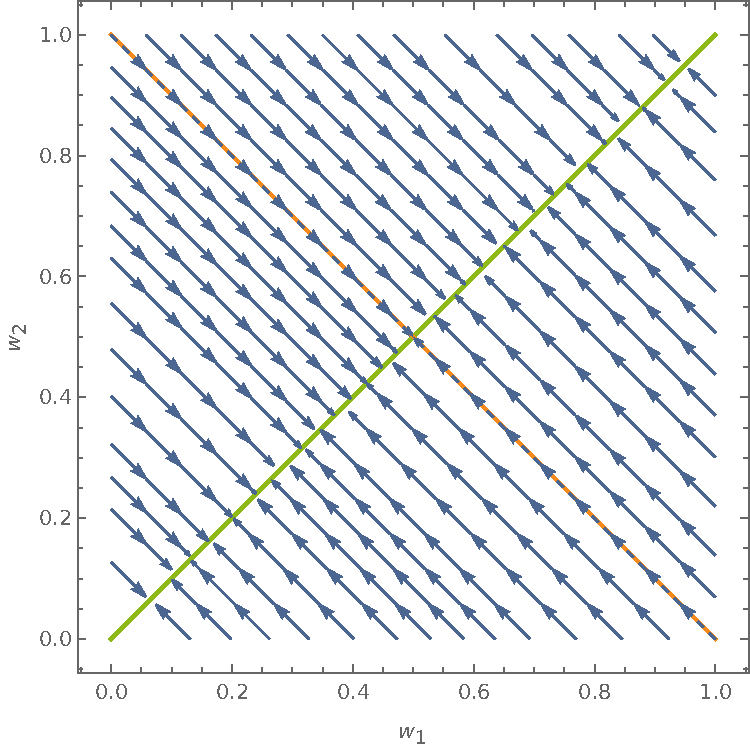
\includegraphics[width=0.45\textwidth]{1-1(a)} \hfill
		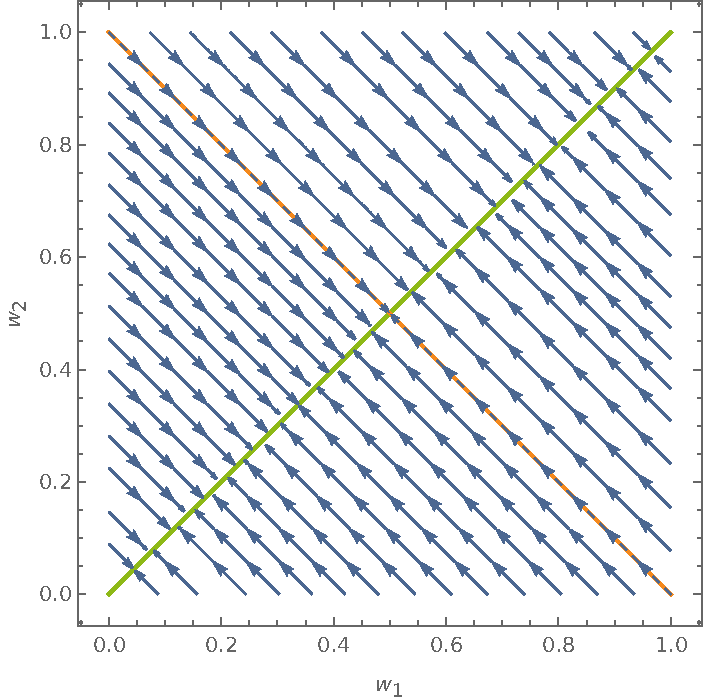
\includegraphics[width=0.45\textwidth]{1-1(b)}
		\caption{Plot of the $(\wq, \ww)$ phase plane indicating trajectories for (left) the nominal system and (right) the system with $t \to -t$.  The normalization $\sumi \wi = 1$ confines the system to the orange line.  The green line represents the equilibrium, which is stable for the nominal system and unstable for the time-reversed system.}
		\label{pplane}
	\end{figure}
	
	Now we will generalize the argument to an $N$-state system.  From Eq.~\refeq{Pauli}, note that
	\al{
		\dwi &= \Pii (\wi - \wi) + \sum{j \neq i}^N \Pij (\wj - \wi)
		= \sum{j \neq i}^N \Pij \wj - \paren{ \sum{j = 1}^N \Pij - \Pii } \wi \\
		&= \sum{j \neq i}^N \Pij \wj + (\Pii - 1) \wi.
	}
	Then $A$ is an $N \times N$ matrix,
	\eqn{A}{
		A = \mqty[
			P_{11} - 1 & P_{12} & P_{13} & \cdots & P_{1N} \\
			P_{21} & P_{22} - 1 & P_{23} & \cdots & P_{2N} \\
			P_{31} & P_{32} & 1 - P_{33} & \cdots & P_{3N} \\
			\vdots & \vdots & \vdots & \ddots & \vdots \\
			P_{N1} & P_{N2} & P_{N3} & \hdots & 1 - P_{NN} ],
	}
	and the generalization of Eq.~\refeq{matrix} is
	\eq{
		\dv{t} \mqty[ w_1 \\ w_2 \\ w_3 \\ \vdots \\ w_N ]
		= \mqty[
			P_{11} - 1 & P_{12} & P_{13} & \cdots & P_{1N} \\
			P_{21} & P_{22} - 1 & P_{23} & \cdots & P_{2N} \\
			P_{31} & P_{32} & 1 - P_{33} & \cdots & P_{3N} \\
			\vdots & \vdots & \vdots & \ddots & \vdots \\
			P_{N1} & P_{N2} & P_{N3} & \hdots & 1 - P_{NN} ]
			\mqty[ w_1 \\ w_2 \\ w_3 \\ \vdots \\ w_N ].
	}
	
	Another method of analyzing stability in applied mathematics is by analyzing the signs of the trace and determinant of $A$~\cite[pp.~136--137]{Strogatz}.  Let $\tau = \Tr(A)$ and $\Del = \det(A)$.  Referring to Eq.~\refeq{A}, clearly $\tau$ is negative (unless it is precisely 0, which would not be very interesting).  For $\Del$, we note that the columns of $A$ are \emph{not} linearly independent due to the normalization constraint on $\Pij$, meaning $A$ is not invertible~\cite{Invertible}.  Thus, it is a singular matrix with zero determinant~\cite{Singular}.
	
	The stability and type of fixed point(s) of the system can be determined using Fig.~\ref{para}~\cite[p.~137]{Strogatz}.  For $\tau < 0$ and $\Del = 0$, the system has a stable non-isolated fixed point, which manifested as a line of stable fixed point in the two-state example.  Due to the normalization condition, the system is confined to a $N - 1$ dimensional region of the $N$ dimensional phase space.  The equilibrium is a generalization of a stable node, so all trajectories in the $N$-dimensional phase space end on the allowed equilibrium point.  Under $t \to -t$, then, the trajectories change direction as in the two-state example.  (This is in contrast to, say, a stable ``center'' whose trajectories are orbits that would change direction under time reversal, but remain stable.)  In other words, \ans{the stable equilibrium becomes an unstable one, so the system described by Eq.~\refeq{Pauli} is time irreversible.} \qed
	
	\begin{figure} \centering
		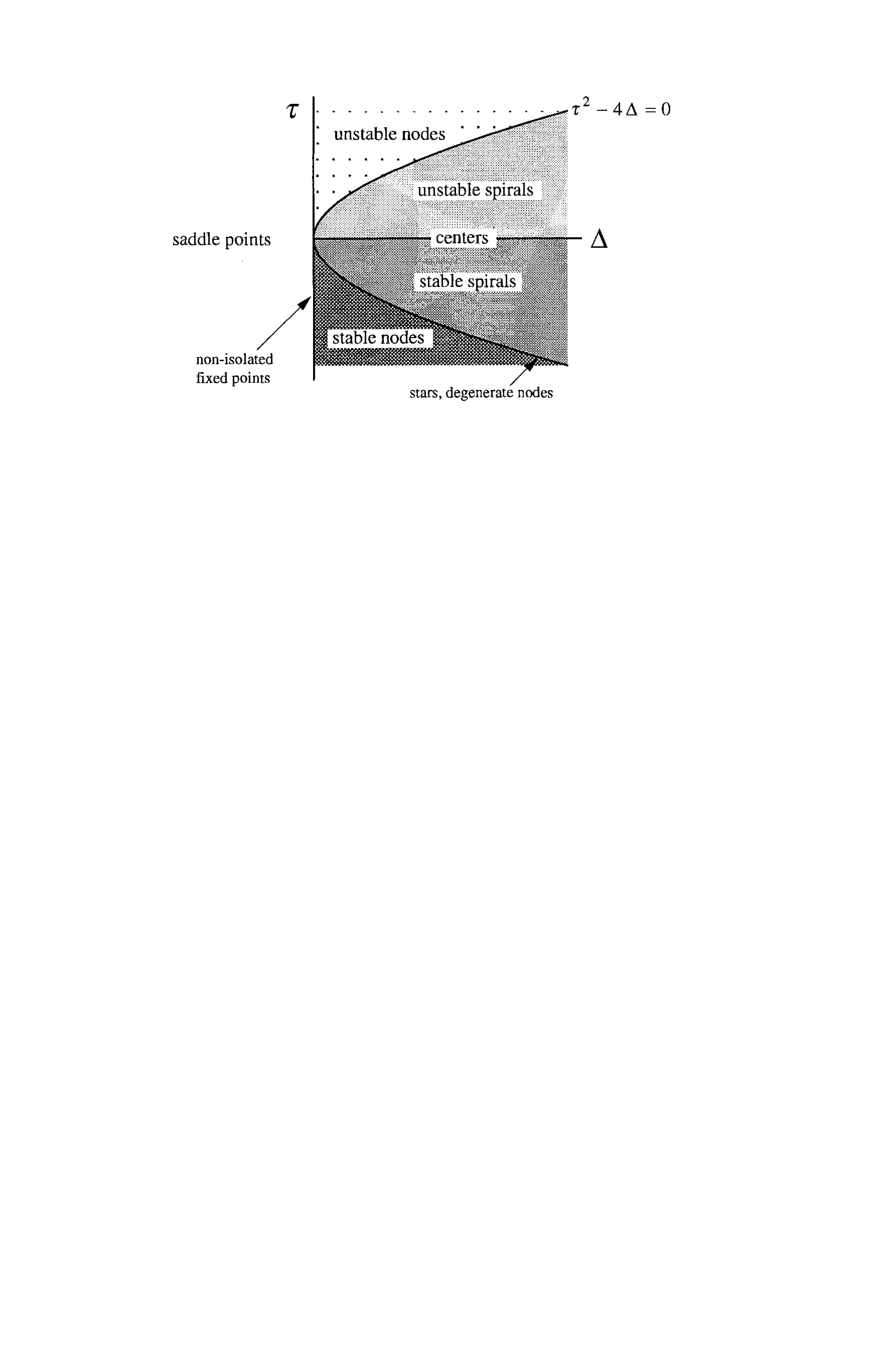
\includegraphics{5-2-8}
		\caption{Fixed point classification scheme using $\tau = \Tr(A)$ and $\Del = \det(A)$~\cite[p.~137]{Strogatz}}
		\label{para}
	\end{figure}
}

%
%	1.1(c)
%
\clearpage
\subprob{
	Show that the entropy $S = -\sumi \wi \ln \wi$ is non-decreasing: $\dS \geq 0$. 
}

\sol{
	Note that
	\eq{
		\dS = -\sumi \dv{t}(\wi \ln \wi)
		= -\sumi \dv{\wi}{t} \dv{\wi}(\wi \ln \wi)
		= -\sumi \dwi (\ln \wi + 1)
		= -\sumi \dwi \ln \wi,
	}
	where we have applied Eq.~\refeq{d0}.  We now apply Eq.~\refeq{Pauli}:
	\eq{
		\dS = -\sumi \sumj (\Pij \wj - \Pji \wi) \ln \wi
		= -\frac{1}{2} \paren{ \sumi \sumj (\Pij \wj - \Pji \wi) \ln \wi + \sumj \sumi (\Pji \wi - \Pij \wj) \ln \wj },
	}
	where we have split the sum in half and swapped indices for the second half.  Then, using the symmetry of $P$,
	\al{
		\dS &= -\frac{1}{2} \sumi \sumj \Pij [ (\wj - \wi) \ln \wi + (\wi - \wj) \ln \wj ]
		= \frac{1}{2} \sumi \sumj \Pij [ (\wi - \wj) \ln \wi - (\wi - \wj) \ln \wj ] \\
		&= \frac{1}{2} \sumi \sumj \Pij (\wi - \wj) (\ln \wi - \ln \wj).
	}
	Since $w_i$ represent probabilities, $0 \leq \wi \leq 1$ for all $i$, which implies $\ln \wi \leq 0$.  If $\wi > \wj$, $\ln \wj$ is more negative than $\ln \wi$.  That is,
	\al{
		\wi \geq \wj &\qimplies \ln \wi - \ln \wj \geq 0 \qq{and} \wi - \wj \geq 0, \\
		\wi \leq \wj &\qimplies \ln \wi - \ln \wj \leq 0 \qq{and} \wi - \wj \leq 0.
	}
	Thus, \ans{$\dS \geq 0$} as desired. \qed
}

%
%	1.2
%

\prob{}{
	{\Renyi} entropy of the order $\alp$ is defined by the formula $\Salp = 1 / (1 -\alp) \ln \sumi \wi^\alp$.
}

%
%	1.2(a)
%

\subprob{
	Show that {\Renyi} entropy of the order 1 is the Boltzmann entropy (in the context of information theory, Boltzmann entropy is called Shannon entropy).
}

\sol{
	Firstly,
	\eq{
		\Salp = \limaq \frac{1}{1 - \alp} \ln \sumi \wi^\alp.
	}
	Note that
	\al{
		\limaq \ln \sumi \wi^\alp &= \ln \sumi \wi
		= \ln(1)
		= 0, &
		\limaq (1 - \alp) &= 0,
	}
	where we have used the result of Prob.~{1.1(a)}.  Applying L'H\^{o}pital's rule, we find
	\eq{
		\limaq \Salp = \limaq \frac{\dv*{(\ln \sumi \wi^\alp)}{\alp}}{\dv*{(1 - \alp)}{\alp}}
		= \limaq -\frac{\dv*{(\sumi \wi^\alp)}{\alp}}{\sumi \wi^\alp}
		= \limaq -\sumi \wi^\alp \ln \wi
		= \ans{ -\sumi \wi \ln \wi, }
	}
	where we have used $\dv*{(a^x)}{x} = (\ln a) a^x$~\cite{Derivative}.  This is the Shannon entropy, as desired.  \qed
}

%
%	1.2(b)
%
\clearpage
\subprob{
	Show that {\Renyi} entropy doesn't decrease: $\dSalp \geq 0$.
}

\sol{
	We note that
	\al{
		\dSalp &= \dv{t}(\frac{1}{1 - \alp} \ln \sumi \wi^\alp)
		= \frac{1}{1 - \alp} \dv{t}(\ln \sumi \wi^\alp)
		= \frac{1}{1 - \alp} \frac{1}{\sumi \wi^\alp} \dv{t}(\sumi \wi^\alp)
		= \frac{1}{1 - \alp} \frac{1}{\sumi \wi^\alp} \alp \sumi \dwi \wi^{\alp - 1} \\
		&= \frac{\alp}{1 - \alp} \frac{\sumi \dwi \wi^{\alp - 1}}{\sumi \wi^\alp}.
	}
	Applying Eq.~\refeq{Pauli} and the same trick as in Prob.~{1.1(c)},
	\al{
		\dSalp &= \frac{\alp}{1 - \alp} \frac{1}{\sumi \wi^\alp} \sumi \wi^{\alp - 1} \sumj (\Pij \wj - \Pji \wi) \\
		&= \frac{\alp}{1 - \alp} \frac{1}{2 \sumi \wi^\alp} \paren{ \sumi \wi^{\alp - 1} \sumj (\Pij \wj - \Pji \wi) + \sumj \wj^{\alp - 1} \sumi (\Pji \wi - \Pij \wj) } \\
		&= \frac{\alp}{1 - \alp} \frac{1}{2 \sumi \wi^\alp} \sumi \sumj \Pij [ \wi^{\alp - 1} (\wj - \wi) + \wj^{\alp - 1} (\wi - \wj) ] \\
%		&= \frac{\alp}{1 - \alp} \frac{1}{2 \sumi \wi^\alp} \sumi \sumj \Pij [ \wi^{\alp - 1} (\wj - \wi) - \wj^{\alp - 1} (\wj - \wi) ] \\
		&= \frac{\alp}{1 - \alp} \frac{1}{2 \sumi \wi^\alp} \sumi \sumj \Pij [ (\wi^{\alp - 1} - \wj^{\alp - 1}) (\wj - \wi) ].
	}
	Keeping in mind that $0 \leq \wi \leq 1$, this result is non-negative in all possible regimes:
	\al{
		\wj \geq \wi \qq{and} \alp < 1
		&\qimplies
		\frac{\alp}{1 - \alp} > 0 \qq{and} \wi^{\alp - 1} - \wj^{\alp - 1} \geq 0 \qq{and} \wj - \wi \geq 0, \\
		\wj \geq \wi \qq{and} \alp > 1
		&\qimplies
		\frac{\alp}{1 - \alp} < 0 \qq{and} \wi^{\alp - 1} - \wj^{\alp - 1} \leq 0 \qq{and} \wj - \wi \geq 0, \\
		\wj \leq \wi \qq{and} \alp < 1
		&\qimplies
		\frac{\alp}{1 - \alp} > 0 \qq{and} \wi^{\alp - 1} - \wj^{\alp - 1} \leq 0 \qq{and} \wj - \wi \leq 0, \\
		\wj \leq \wi \qq{and} \alp > 1
		&\qimplies
		\frac{\alp}{1 - \alp} < 0 \qq{and} \wi^{\alp - 1} - \wj^{\alp - 1} \geq 0 \qq{and} \wj - \wi \leq 0.
	}
	Of course $\sumi \wi^\alp > 0$ in any case.  Thus, \ans{$\dSalp \geq 0$} as desired. \qed
}